\documentclass[tikz,border=10pt]{standalone}
\usepackage{tikz}
\usetikzlibrary{shapes, arrows.meta, positioning, fit, calc, backgrounds, shadows}

% --- 配色 ---
\definecolor{cOld}{RGB}{100, 100, 100}   % 灰色:旧时代
\definecolor{cNav}{RGB}{33, 150, 243}    % 蓝色:导航/切换
\definecolor{cFile}{RGB}{230, 81, 0}     % 橙色:文件操作

\tikzset{
    font=\sffamily,
    % 核心节点
    cmdNode/.style={
        rectangle, rounded corners=6pt, thick,
        minimum width=3.5cm, minimum height=1.2cm,
        align=center, drop shadow={opacity=0.1},
        font=\bfseries\large
    },
    % 连线标签
    labelNode/.style={
        fill=white, inner sep=2pt, font=\footnotesize\color{gray!80}, align=center
    },
    % 箭头
    conn/.style={
        ->, >=Latex, thick, draw=gray!60, rounded corners=10pt
    }
}

\begin{document}
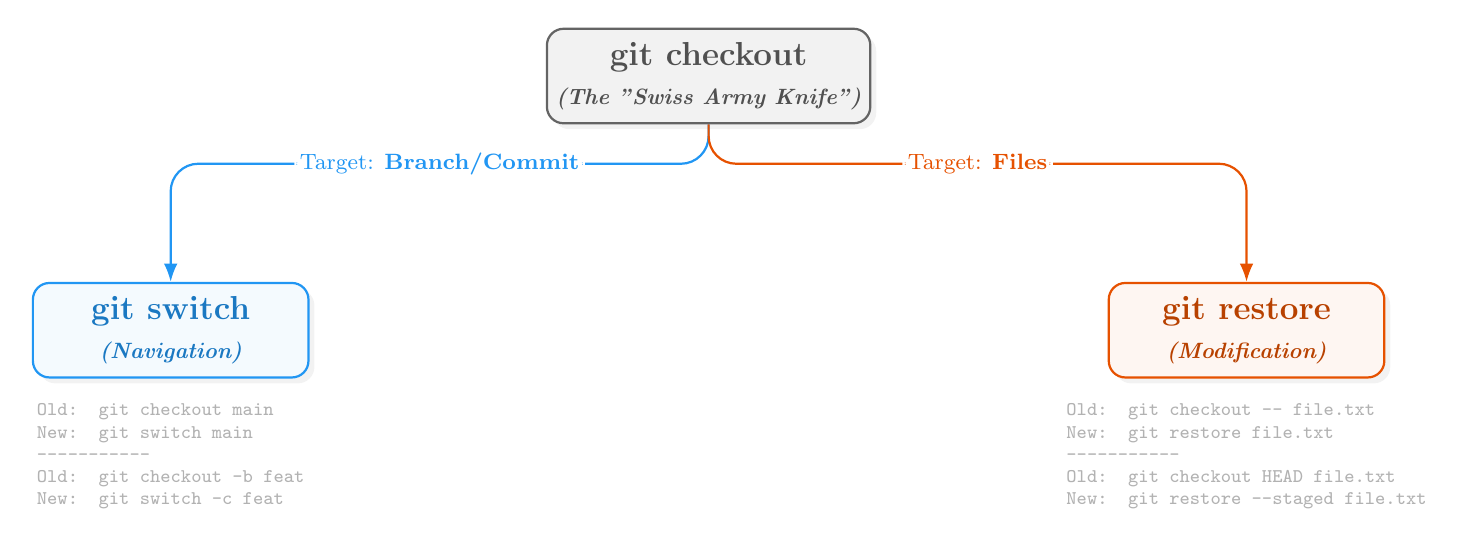
\begin{tikzpicture}[node distance=2.0cm and 3.0cm]

	% 1. 旧皇:Git Checkout
	\node[cmdNode, draw=cOld, fill=gray!10, text=cOld!80!black] (checkout) {
		git checkout\\
		\footnotesize \itshape (The "Swiss Army Knife")
	};

	% 2. 新王左:Switch (导航)
	\node[cmdNode, draw=cNav, fill=cNav!5, text=cNav!80!black, below left=of checkout] (switch) {
		git switch\\
		\footnotesize \itshape (Navigation)
	};

	% 3. 新王右:Restore (文件)
	\node[cmdNode, draw=cFile, fill=cFile!5, text=cFile!80!black, below right=of checkout] (restore) {
		git restore\\
		\footnotesize \itshape (Modification)
	};

	% 4. 连线与对比

	% Left Path
	\draw[conn, cNav] (checkout.south) -- ++(0,-0.5) -| (switch.north)
	node[pos=0.25, labelNode, text=cNav] {Target: \textbf{Branch/Commit}};

	% Right Path
	\draw[conn, cFile] (checkout.south) -- ++(0,-0.5) -| (restore.north)
	node[pos=0.25, labelNode, text=cFile] {Target: \textbf{Files}};

	% 5. 详细语法对比框

	% Switch Box
	\node[below=0.2cm of switch, align=left, font=\scriptsize\ttfamily, text=gray!60] (descSwitch) {
		\textbf{Old:} git checkout main\\
		\textbf{New:} git switch main\\
		-----------\\
		\textbf{Old:} git checkout -b feat\\
		\textbf{New:} git switch -c feat
	};

	% Restore Box
	\node[below=0.2cm of restore, align=left, font=\scriptsize\ttfamily, text=gray!60] (descRestore) {
	\textbf{Old:} git checkout -{}- file.txt\\
	\textbf{New:} git restore file.txt\\
	-----------\\
	\textbf{Old:} git checkout HEAD file.txt\\
	\textbf{New:} git restore -{}-staged file.txt
	};

\end{tikzpicture}
\end{document}